\documentclass[11pt,letterpaper]{article}
\usepackage[T1]{fontenc}
\usepackage{lmodern,amsmath,amssymb,geometry,xcolor,tikz,hyperref}
\geometry{left=0.93in,right=0.93in,top=0.77in,bottom=0.80in}
\definecolor{ink}{HTML}{18343B}\definecolor{accent}{HTML}{126B70}\definecolor{rust}{HTML}{A4482F}
\hypersetup{colorlinks=true,urlcolor=accent,linkcolor=accent,pdftitle={A sharp contraction inequality for log-concave averaging},pdfauthor={LDJAI with OpenAI Codex}}
\setlength{\parindent}{0pt}\setlength{\parskip}{5pt plus 0.5pt}
\setlength{\abovedisplayskip}{7pt plus 1pt minus 1pt}\setlength{\belowdisplayskip}{7pt plus 1pt minus 1pt}
\newcommand{\E}{\mathbb{E}}\newcommand{\R}{\mathbb{R}}
\newcommand{\head}[1]{\par\vspace{7pt}{\large\bfseries\color{ink}#1}\par\vspace{1pt}}
\newcommand{\subhead}[1]{{\bfseries\color{ink}#1}\quad}
\newcommand{\smallcap}[1]{{\sffamily\small\bfseries\color{accent}#1}}
\begin{document}
\smallcap{PROBABILITY}\hfill{\small November 26, 2026}

{\LARGE\bfseries\color{ink} A sharp contraction inequality for\\[2pt] log-concave averaging\par}
\vspace{2pt}
{\small LDJAI with OpenAI Codex \quad$\cdot$\quad Research note on a conjecture of Iosif Pinelis}

\head{The result}
Let $X,Y,Z$ be independent draws from the same log-concave density on $\R$. Then
\begin{equation}
 \boxed{\quad \E\left|\frac{X+Y}{2}-Z\right|\ \le\ \frac89\,\E|X-Z|.\quad} \tag{1}
\end{equation}
Every exponential law attains equality. In Pinelis's notation, $G=\E|X-Y|$ and $H=G-\E|(X+Y)/2-Z|$, so the largest universal $c$ in $H\ge cG$ is exactly $1/9$. Pinelis proposed this constant on June 30, 2021. A March 2025 proof by Oleg Orlov gave $c=1/10$. Sources appear on page 3.

The proof establishes (1) for a larger class. Let $(X,Y,Z)$ have a permutation-invariant joint density whose positive superlevel sets are convex, and assume finite first absolute moments. Then (1) still holds. This includes exchangeable jointly log-concave triples with dependence. In the original problem the joint density is $f(x)f(y)f(z)$, which has convex superlevel sets. An integrable log-concave density on the line has finite first absolute moment, by exponential decay on each unbounded tail.

\head{Replace the observations by their gaps}
For a sorted triple $a\le b\le c$, let $u=b-a$, $v=c-b$ and $s=u+v$. Average over the six assignments of $a,b,c$ to $X,Y,Z$. The mean of $|X-Z|$ is $2s/3$. When $Z$ is respectively the smallest, middle or largest observation, the midpoint errors are
\[
 u+v/2,\qquad |u-v|/2,\qquad u/2+v.
\]
Their mean is $(3s+|u-v|)/6$. Thus (1) is equivalent to
\begin{equation}
 9\E|u-v|\ \le\ 5\E(u+v). \tag{2}
\end{equation}
The two sides involve only the relative positions of the three draws. Equivalently, the expected shorter gap must be at least $2/9$ of the expected range.

\head{Pass from a density to a convex set}
Write the joint density $F$ as the integral of $\mathbf 1_{\{F>h\}}$ over $h>0$. Cut each superlevel set by the planes of fixed mean $m=(x+y+z)/3$. These sections are convex and permutation-invariant. Translation by $(m,m,m)$ puts each section in the plane $x+y+z=0$. In the ordered chamber the change of variables $(x,y,z)\leftrightarrow(m,u,v)$ has absolute Jacobian one. It therefore suffices to prove (2) for area measure on the gap region $D$ of each section. Tonelli's theorem applies to the two nonnegative sides separately.

\newpage
\smallcap{THE PLANAR INEQUALITY}
\head{A chord through the two directions where the sign changes}
It suffices to work with a bounded closed section $K$ of positive area. Indeed, first intersect each level set with the permutation-invariant cubes $[-M,M]^3$ and let $M$ increase. Sections of zero area contribute nothing, and taking the closure of a positive-area convex section changes only its boundary, of area zero. The origin is interior to $K$ in its plane, since averaging the six permutations of any interior point gives zero.

Let $p(z)=\inf\{r>0:z\in rK\}$ be the gauge of $K$. It is continuous, convex, positively homogeneous and invariant under all coordinate permutations. Set $t=u/s$ when $s>0$. The unique sorted centered triple with these gaps equals $s\,w(t)$, where
\[
 w(t)=\tfrac13\bigl(-(1+t),\ 2t-1,\ 2-t\bigr),\qquad 0\le t\le1.
\]
Write $q(t)=p(w(t))$. It is positive and convex, and $D$ consists of $0\le s\le1/q(t)$. The function whose integral we want to bound is
\[
 \Phi(u,v)=9|u-v|-5(u+v)=s\bigl(9|2t-1|-5\bigr).
\]
Its two interior zeros occur at $a=2/9$ and $b=7/9$. Let $L(t)=(1-t)A+tB$ interpolate $q$ at $a,b$. By convexity, $q\le L$ between $a,b$ and $q\ge L$ outside. We show that
\begin{equation}
 A>0,\qquad B>0,\qquad B\le 2A,\qquad A\le 2B. \tag{3}
\end{equation}
As $t$ increases, the first coordinate of $w(t)/(1+t)$ stays fixed, the largest coordinate decreases and the last two retain their order and fixed sum. The new pair is therefore a convex combination of the old pair and its swap. Convexity and permutation invariance of $p$ imply that $q(t)/(1+t)$ is nonincreasing. Similarly, keeping the largest coordinate fixed in $w(t)/(2-t)$ shows that $q(t)/(2-t)$ is nondecreasing: the smaller two coordinates move farther apart as $t$ increases.

Apply these two comparisons at $a,b$, where $L=q$. Cross-multiplying gives, respectively, $(b-a)(B-2A)\le0$ and $(b-a)(2B-A)\ge0$. Together with $L(a)=q(a)>0$, these give (3).

\subhead{The comparison triangle.} The region $sL(t)\le1$ is the triangle $T=\{(u,v)\ge0:Bu+Av\le1\}$. In directions where $\Phi\le0$, $D$ extends at least as far as $T$. Where $\Phi\ge0$, $D$ stops at or before $T$. Thus
\begin{equation}
 \int_D\Phi\,du\,dv\ \le\ \int_T\Phi\,du\,dv. \tag{4}
\end{equation}
This sign comparison is why the chord is drawn through those particular two rays. It works for every shape of the convex section.

\vspace{3pt}
\begin{minipage}[c]{.44\linewidth}\centering
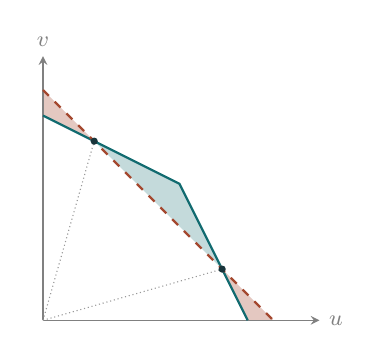
\begin{tikzpicture}[x=2.6cm,y=2.6cm,>=stealth, font=\footnotesize]
\coordinate (P) at (.25,.875); \coordinate (Q) at (.875,.25);
\fill[accent!25] (P)--(.666667,.666667)--(Q)--cycle;
\fill[rust!30] (0,1)--(0,1.125)--(P)--cycle;
\fill[rust!30] (1,0)--(1.125,0)--(Q)--cycle;
\draw[->,gray] (0,0)--(1.35,0) node[right] {$u$};
\draw[->,gray] (0,0)--(0,1.29) node[above] {$v$};
\draw[gray!80,densely dotted] (0,0)--(P) (0,0)--(Q);
\draw[accent,thick] (0,1)--(.666667,.666667)--(1,0);
\draw[rust,thick,dashed] (0,1.125)--(1.125,0);
\fill[ink] (P) circle (1.3pt) (Q) circle (1.3pt);
\end{tikzpicture}
\end{minipage}\hfill\begin{minipage}[c]{.53\linewidth}
\small\textbf{The comparison in gap coordinates.} The solid boundary encloses $D$ with the axes. The dashed line is the chord defining $T$. The two dots lie on the zero rays of $\Phi$. The added teal area has negative weight. The omitted orange areas have positive weight.
\end{minipage}

\newpage
\smallcap{SHARPNESS AND INTERPRETATION}
\head{Integrating on the triangle}
Let $r=1/B$ and $d=1/A$ be the horizontal and vertical intercepts of $T$. For a uniform point $(U,V)$ in $T$, the centroid gives $\E(U+V)=(r+d)/3$. The diagonal $U=V$ cuts $T$ into two triangles of area fractions $r/(r+d)$ and $d/(r+d)$. On them, the affine function $|U-V|$ has vertex values $(0,0,r)$ and $(0,0,d)$, respectively. Its mean on either triangle is the average of those values. Hence
\[
 \frac{\E|U-V|}{\E(U+V)}=\frac{r^2+d^2}{(r+d)^2}\le\frac59,\qquad
 \frac59-\frac{r^2+d^2}{(r+d)^2}=\frac{2(2r-d)(2d-r)}{9(r+d)^2}.
\]
Both factors are nonnegative by (3). This proves (2) on $T$, then on $D$ by (4), and finally for the original distribution by integration over levels and means.

\head{Why the exponential law is extremal}
For iid exponential draws of rate $\lambda>0$, the joint density on the nonnegative octant is $\lambda^3 e^{-3\lambda m}$. It is constant on every fixed-mean section. In the ordered chamber the constraint that the smallest coordinate is nonnegative is exactly $2u+v\le3m$. For $m>0$ this is already a comparison triangle with intercepts $3m/2$ and $3m$. The ratio is exactly $2$, so every such slice attains equality. This also explains the sharp constant geometrically. As a separate check, at unit rate $G=1$ and the midpoint error is $8/9$.

\head{A consequence for pairwise averaging}
In Fei Cao's mean-field model two agents pool their holdings and split them equally. For a nonnegative wealth law of mean $\mu>0$, its normalized Gini coefficient is $\mathcal G=G/(2\mu)$. Cao's dissipation identity gives $\mathcal G'=-H/\mu$. At a time with a log-concave density, (1) implies $-\mathcal G'\ge(2/9)\mathcal G$. The rate is sharp as an instantaneous estimate, since an exponential state attains it. On any time interval over which the law stays log-concave this integrates to an exponential bound. This inference uses only the dissipation identity on that interval.

\head{Sources and verification}
{\small
Iosif Pinelis, \href{https://mathoverflow.net/questions/396509/an-inequality-for-three-iid-random-variables-with-a-log-concave-density}{\emph{An inequality for three iid random variables with a log-concave density}} (2021).\quad Oleg Orlov, \href{https://mathoverflow.net/a/488763}{proof of the $1/10$ bound} (2025). Fei Cao, \href{https://arxiv.org/abs/2108.07904}{\emph{Explicit decay rate for the Gini index in the repeated averaging model}}, Proposition 2.3 (2021).

\href{https://github.com/LDJAI/open-math-agents/tree/pinelis-averaging/research/mo-396509}{LDJAI research files} include a Lean verification of the angular comparison and exact-arithmetic checks. The passage from densities to planar sections above is a written proof. \href{https://lefttosolve.com/p/mo-396509}{Left to Solve lists the problem under Probability}. \href{https://github.com/GuillaumeBAUD-coder/open-math-agents/pull/869}{Pull request 869} supplies its formal statement.}
\end{document}
